\documentclass{article}

\usepackage{amsmath}
\usepackage{amsfonts}
\usepackage{amssymb}
\usepackage{graphicx}
\usepackage[margin=0.7in]{geometry}
\usepackage{booktabs}
\usepackage{multirow}
\usepackage{multicol}

\title{Assignment 6}
\author{Miguel A. Gomez B.}

\begin{document}
	\maketitle
\section{Testing a Sequence of Numbers.}
\paragraph{}\textit{(50 Points)} Together with this assignment you will find a sequence of $100.000$ numbers (\textit{'Sequence.txt'}) generated with the brand new \textit{PPP} algorithm. Your task will be to test if the algorithm passes the following tests:
\begin{itemize}
	\item Spectral tests. (In order to perform this test assume that the algorithm used is \textit{MRG32k3a} by L'Ecuyer).
	\item $\chi^2$ Test.
	\item Kolmogorov-Smirnov Test.
\end{itemize}
\paragraph{Solution}Before we proceed with the tests we want to get an idea of how the data is distributed.
\begin{center}
	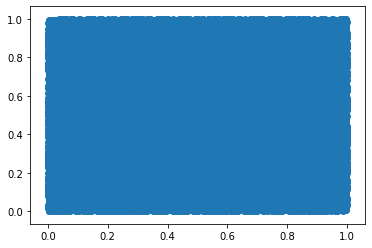
\includegraphics[width=0.5\linewidth]{distribution.png}
\end{center}
\paragraph{}And descriptive statistics gives us an idea about dispersion and uniformity,
\begin{table}[h!]
	\begin{center}
		\label{tab:table1}
		\begin{tabular}{|l|r|}
			\hline
			\textbf{Statistic} & \textbf{Value}\\
			\hline
			Mean & 0.5\\
			Median & 0.501\\
			Mode & 0.565\\
			Standard Deviation & 0.288\\
			Max & 0.999\\
			Min & 4.243e-05\\
			\bottomrule
		\end{tabular}
		\caption{Descriptive Statistics}
	\end{center}
\end{table}
\paragraph{}As we can see in the graph it seems  uniform, the mean and the median, confirms that, but the standard deviation tells us a different story that it is not visible from the graph, if the data is between 0 and 1 with an average difference of $0.288$, it seems suspicious about how the data is distributed, we will a histogram.
\begin{center}
	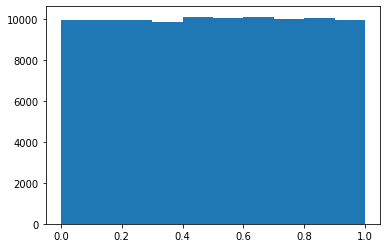
\includegraphics[width=0.5\linewidth]{histogram.png}
\end{center}
\paragraph{} Now we see that there is uniformity between the data,but also we can see differences between intervals, in any case, we see that the data is closely related to a uniform distribution, the tests will determine numerically how uniform these generated values and as a consequence the algorithm that generate them.
\subsection{Spectral Test (Not finished).}
\subsubsection{2D}
\begin{center}
	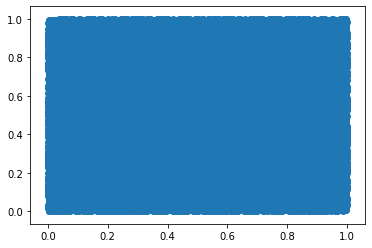
\includegraphics[width=0.5\linewidth]{2d_scatter.png}
\end{center}
\subsection{3D}
\begin{center}
	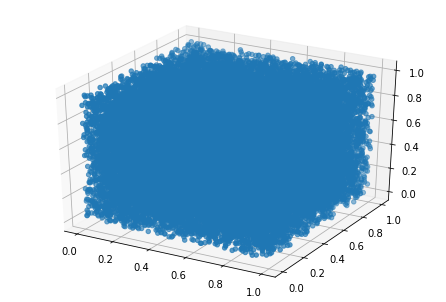
\includegraphics[width=0.5\linewidth]{3d_scatter.png}
\end{center}
\subsection{$\chi^2$ Test.}
On the $\chi^2$ test, we compute $\chi^2$ with the following equation
\begin{equation}
\chi^2 = \sum_{i=1}^{n} \frac{(O_i - E_i)^2}{E_i},
\end{equation}
\paragraph{}where $n$ is the number of intervals, $O_i$ is the observed value and $E_i$ is the expected value. Then we lookup on the $\chi^2$ table for an $\alpha=0.05$(generally) and an $n-1$ degrees of freedom. And formulate a hypothesis(\textit{Null Hypothesis}): There is no difference between our computed distribution (the generated numbers) and the theoretical distribution. If the sum is less than $\chi^2_{[1-\alpha;n-1]}$, then the hypothesis previous hypothesis cannot be rejected at the level of significance $\alpha$:
$$\sum_{i=1}^{n} \frac{(O_i - E_i)^2}{E_i} < \chi^2_{[1-\alpha;n-1]}$$
\paragraph{}Using the information computed from the following histogram
\begin{center}
	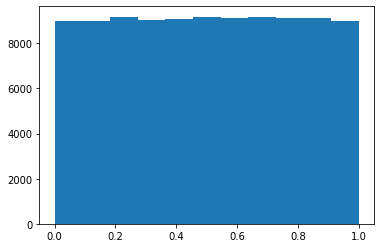
\includegraphics[width=0.5\linewidth]{histogram2.png}
\end{center}
\paragraph{}we choose our $n=11$ and to formulate an expected value for every bin, we state that the expected value is $\frac{100000/11} \approx 9090.90$, because we are assuming that the values are related to a uniform distribution.
\newpage
\paragraph{} The following results resume our computation for $\chi^2$
\begin{table}[h!]
	\begin{center}
		\begin{tabular}{|c|c|c|c|}
			\hline
			\textbf{Interval} & \textbf{$E_i$} & \textbf{$O_i$} & $\frac{(O_i - E_i)^2}{E_i}$\\
			\hline
			1 & 9090.90 & 9007 & 0.77448091\\
			2 & 9090.90 & 8997 & 0.97008091\\
			3 & 9090.90 & 9157 & 0.48048091\\
			4 & 9090.90 & 9041 & 0.27400091\\
			5 & 9090.90 & 9066 & 0.06825091\\
			6 & 9090.90 & 9163 & 0.57168091\\
			7 & 9090.90 & 9126 & 0.13545091\\
			8 & 9090.90 & 9181 & 0.89280091\\
			9 & 9090.90 & 9113 & 0.05368091\\
			10 & 9090.90 & 9143 & 0.29848091\\
			11 & 9090.90 & 9006 & 0.79305091\\
			\hline
			\multicolumn{3}{|c|}{$\chi^2$} & 5.312\\
			\hline
		\end{tabular}
		\caption{Computation of $\chi^2$}
	\end{center}
\end{table}
\paragraph{}Now we compare our $\chi^2$ compared with  the value on the table, for a $\nu = 11 - 1 = 10$, and $p = 1 - 0.05$ is $18.31$, as we can see $5.312 < 18.31$ so the hypothesis cannot be rejected at least with a level of significance of $0.05.$
\begin{center}
	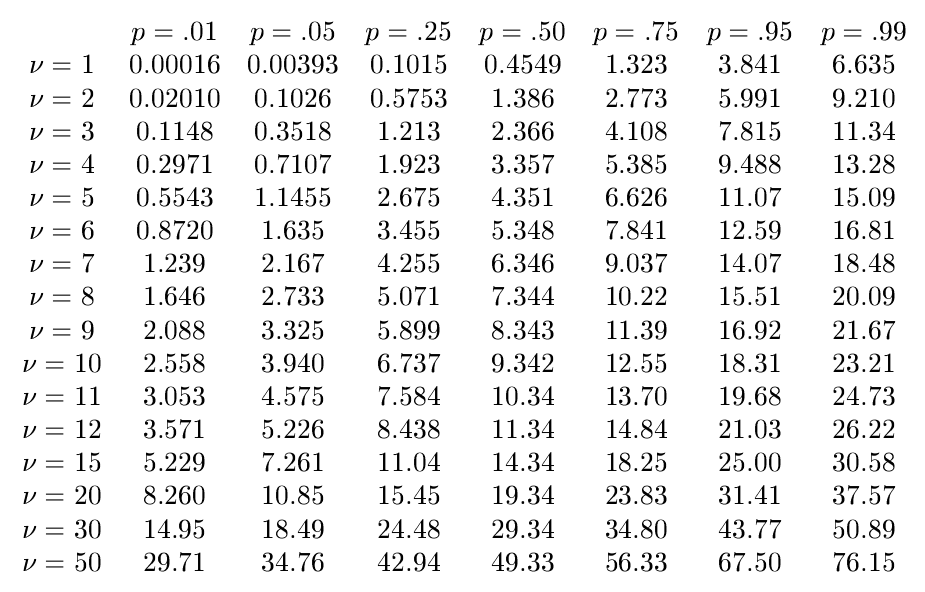
\includegraphics[width=0.7\linewidth]{chi_table.png}
\end{center}
\paragraph{}As we can see, our computed value lies between $p=.05$ and  
\subsection{Kolmogorov-Smirnov Test.}
On this test we will compare the PDF (Probability Density Function), $F(X)$, against an empirical PDF uniform distribution, $S_n(X)$ from a sample of $N$ observations, then, by definition,
$$F(x) = x, 0 \leq x \leq 1$$
\begin{equation}
S_n(x) = \frac{R_1, R_2, R_3, \dots, R_n \leq x}{N}
\end{equation}
\paragraph{} where $R_n$ is an observation. The test also requires us to sort the observations and compute $D^{+}$ and $D^{-}$,
$$D^{+} = \max_{1 \leq i \leq N} \left[ \frac{i}{n} - R_i \right], D^{-} = \max_{1 \leq i \leq N} \left[ R_i - \frac{i-1}{n}\right],$$
\paragraph{} Then we compute $D$ as
$$D = \max(D^{+}, D^{-}),$$
\paragraph{} and same as before we find our correspondent value on the KS table, with the expected level of significance(as before we will use $\alpha= 0.05$), if our value is less that the value founded, we accept the null hypothesis(The data may be was generated from an uniform distribution).
\paragraph{}Same as before we will use the bin values obtained from the previous histogram. And therefore we compute $D^{+}$ and $D^{-}$ with $F(x_i)$ defined as:
$$F(x_i) = \frac{1}{b-a}, a \leq x \leq b,$$
\paragraph{}with $a=0$ and $b=1$. Then $F(x)=x$. Now sorting the values, the following table resumes our computations:
\begin{table}[h!]
	\begin{center}
		\begin{tabular}{|c|c|c|c|c|}
			\hline
			\textbf{i} & \textbf{$F(x_i)$} & \textbf{$i/n$} & $i/n - F(x_i)$ & $F(x_i) - (i-1)/n$\\
			\hline	
			1 & 4.24310000e-05 & 0.08333333 & 8.32909023e-02 & 4.24310000e-05\\
			2 & 9.09467555e-02 & 0.16666667 & 7.57199112e-02 & 7.61342212e-03\\
			3 & 1.81851080e-01 & 0.25 & 6.81489201e-02 & 1.51844132e-02\\
			4 & 2.72755404e-01 & 0.33333333 & 6.05779290e-02 & 2.27554044e-02\\
			5 & 3.63659729e-01 & 0.41666667 & 5.30069378e-02 & 3.03263955e-02\\
			6 & 4.54564053e-01 & 0.5 & 4.54359467e-02 & 3.78973866e-02\\
			7 & 5.45468378e-01 & 0.58333333 & 3.78649556e-02 & 4.54683777e-02\\
			8 & 6.36372702e-01 & 0.66666667 & 3.02939645e-02 & 5.30393688e-02\\
			9 & 7.27277027e-01 & 0.75 & 2.27229734e-02 & 6.06103600e-02\\
			10 & 8.18181351e-01 & 0.83333333 & 1.51519822e-02 & 6.81813511e-02\\
			11 & 9.09085676e-01 & 0.91666667 & 7.58099112e-03 & 7.57523422e-02\\
			12 & 9.99990000e-01 & 1. & 1.00000000e-05 & 8.33233333e-02\\
			\hline
			\multicolumn{3}{|c|}{} & $D^+ = 0.08329090233333333$ & $D^- = 0.08332333333333342$\\
			\hline
			\multicolumn{5}{|c|}{$D = \max(D^+, D^-) = 0.08332333333333342$}\\
			\hline
		\end{tabular}
		\caption{KS Test computation}
	\end{center}
\end{table}
\paragraph{}Now we compare our result against the KS Table:
\begin{center}
	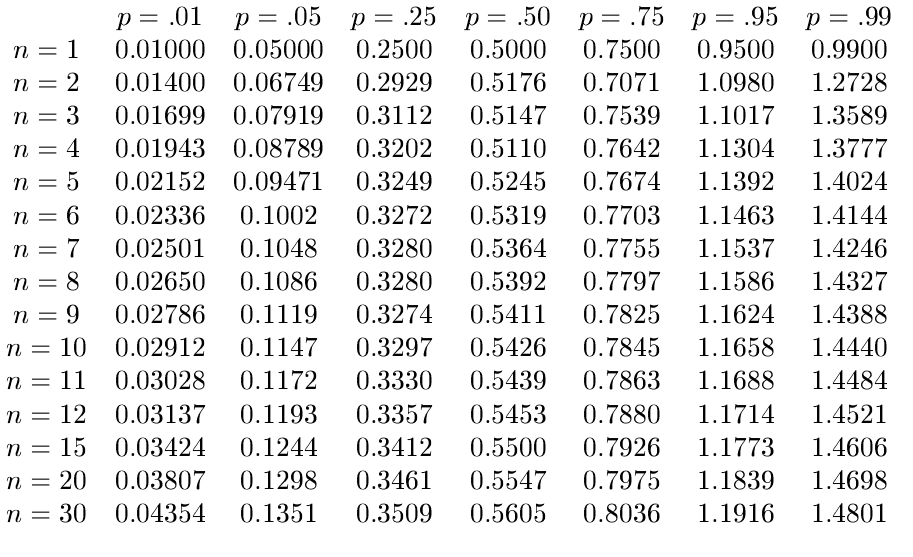
\includegraphics[width=0.7\linewidth]{KS_table.png}
\end{center}
\paragraph{}same as before the test is passed if $D < K_{[1-\alpha=0.95;n=12]}$, some authors like Knuth, even compare $D^+$ and $D^-$, and as we see:
$$0.083 < 1.17,$$
\paragraph{} Which satisfies both conditions and the test is passed.
\end{document}